%!TEX root = ../main.tex

\chapter{Schematic Editor}

The first step in every project is schematic capture.
If this term is unfamiliar, we are referring to the process of laying out the components and connections between them in logical, well-defined fashion.
You may have only the barest idea of the circuit aspects or you may have the major aspects already sketched on paper;
whatever your situation, transferring the schematic into KiCad begins with the Schematic Editor.

Before we dive into the simplistic aspects of the schematic editor, it will pay us dividends later to properly understand how the schematic editor views more complex schematics.
This will allow you to structure the schematic in your mind more closely to how Schematic Editor expects.

\section{Hierarchical Schematics Explained}

The basic, underlying paradigm of the Schematic Editor is the idea of \textit{hierarchical schematics}.
If the overall schematic represents the full circuit that will exist on the circuit board at the end of production, then the hierarchy provides a logical grouping of similar component sets.
This allows you to reuse common subsets throughout your design.
The hierarchy also explicitly structures your schematics as a top-down tree.
\begin{figure}
	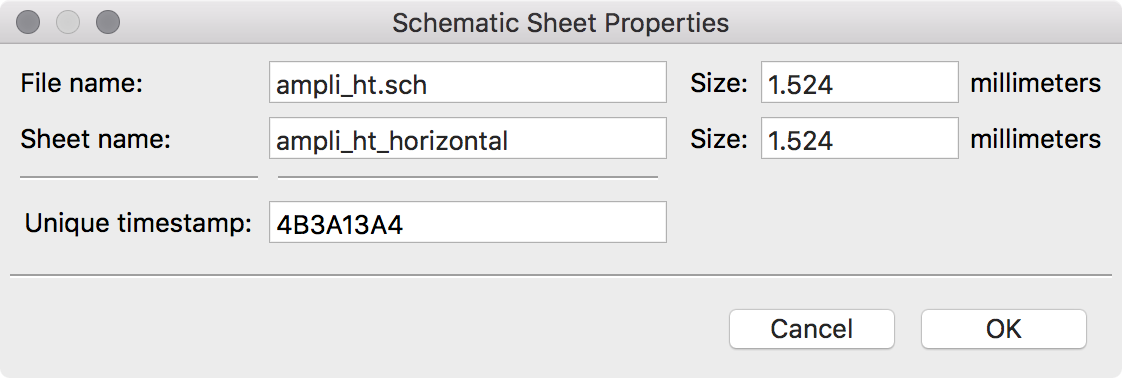
\includegraphics{chapter5/subsheet.png}
	\caption[Sub-Sheets]{The subsheet dialog specifies the file name, sheet name and a unique timestamp.}
\end{figure}

At the root of the tree, is the first schematic sheet you open, usually with the same name as your project and the extension `\textbf{.sch}'.
Off of this root, you can create \textit{sub-sheets} that are placed in the root sheet.
The sub-sheet has both a ``File name'' and a ``Sheet name''.
The File name is the name of the sub-sheet on the underlying filesystem.
This is the name you will see if you open your project folder outside of KiCad.
The Sheet name is the internal reference of the specific \textit{instance} of the sub-sheet in KiCad.

One of the primary benefits of this setup is the ability to organize the relationship between subsheets.
Instead of utilizing global net labels to connect disparate elements between sheets, you can use hierarchical subsheets layout the explicit connection between schematic elements.

It can also allow you to create and re-use common elements through and between projects.
This will be useful when we begin discussing design reuse in section \ref{sec:reuse}.



\section{Understanding the Schematic Editor}

When you first open the schematic editor, you are presented with a blizzard of information.
In KiCad, the majority of functions are accessed using buttons and hotkeys.
Unlike many programs, where functionality is often buried in sub-menus, KiCad prefers to expose its controls up front.
This has the benefit of providing easy access to virtually all commands, and the drawback of an overwhelming first impression.

\begin{figure}
	\hspace*{-1cm}%
	\begin{tikzpicture}[baseline]
	\begin{scope}
		\node[anchor=south west,inner sep=0] (image) at (0,0) 
			{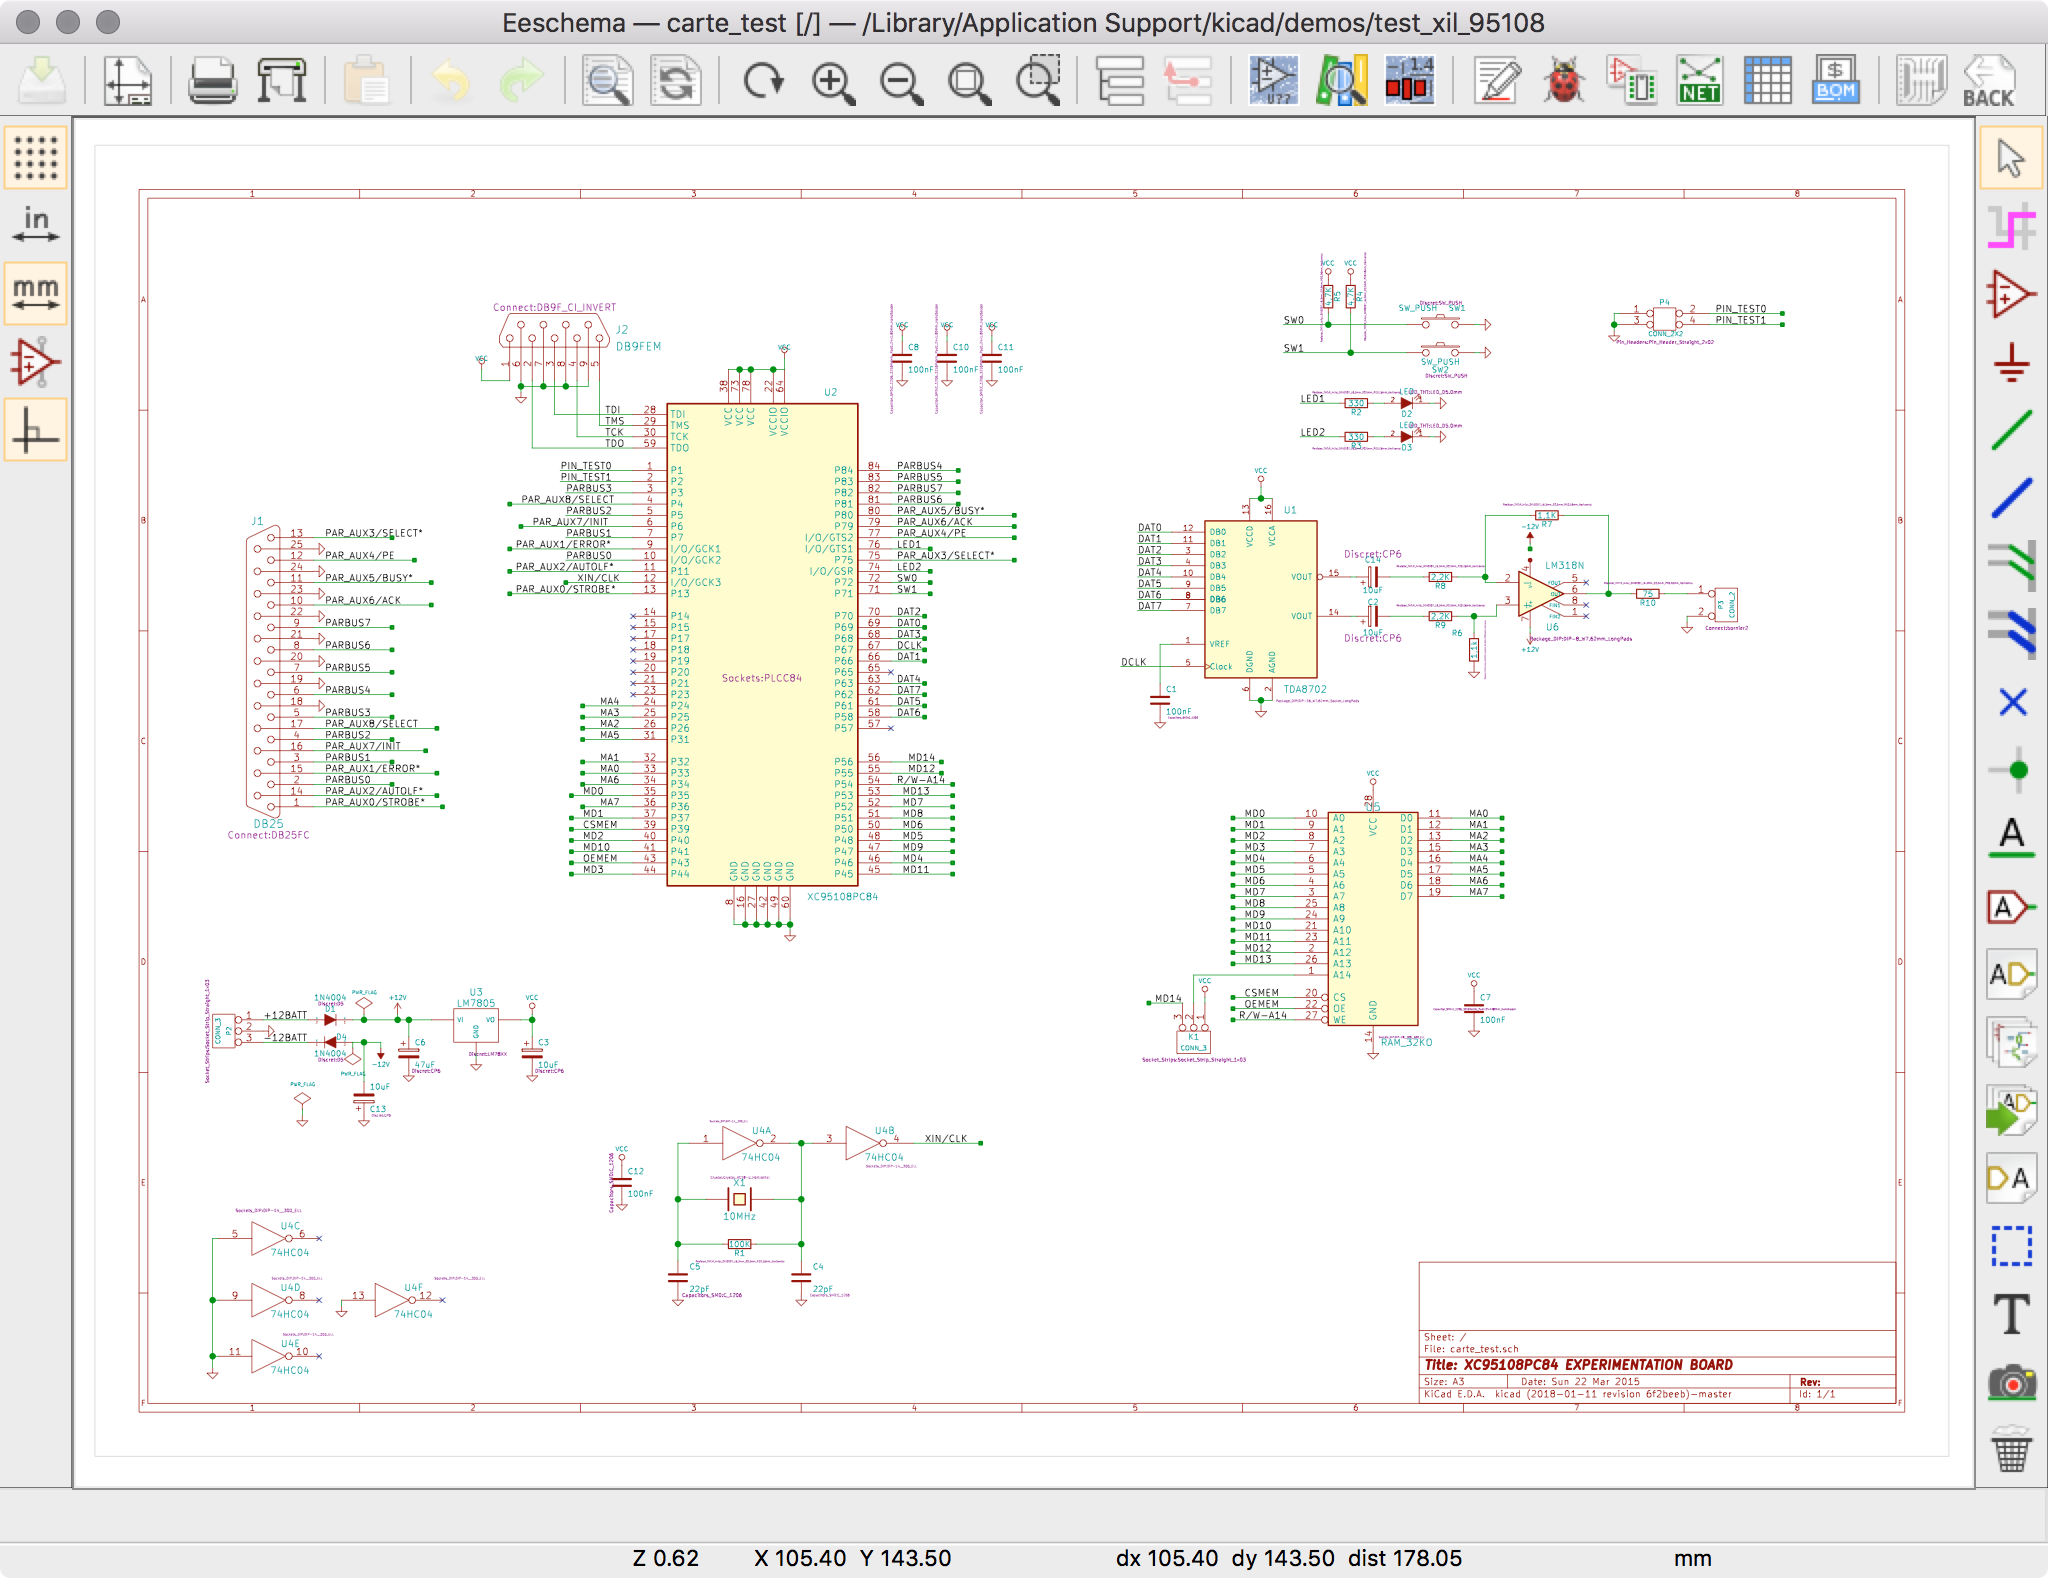
\includegraphics[width=4.0in]{chapter5/eeschema-main.png}};
		\begin{scope}[x={(image.south east)},y={(image.north west)}]
			\node [anchor=south] (file) at (0.08,1.0) {\large File\strut };
			\node [anchor=south] (edit) at (0.2575,1.0) {\large Edit\strut };
			\node [anchor=south] (view) at (0.438,1.0) {\large View\strut };
			\node [anchor=south] (app) at (0.763,1.0) {\large Applications\strut };
			\node [anchor=south, rotate=-90] (tools) at (1.0,0.5) {\large Schematic Tools};
			\node [anchor=north, rotate=-90] (options) at (0.0,0.5) {\large Display Options};
			\node [anchor=north west] (coord) at (0.0,0.0) {\large Coordinates };
			
%			\draw[help lines,xstep=.05,ystep=.05] (0,0) grid (1,1);
			\draw[red,thick,rounded corners] (0.0,0.923) rectangle (0.155,0.97);
			\draw[red,thick,rounded corners] (0.162,0.923) rectangle (0.35,0.97);
			\draw[red,thick,rounded corners] (0.357,0.923) rectangle (0.525,0.97);
			\draw[red,thick,rounded corners] (0.60,0.923) rectangle (1.0,0.97);
			\draw[black!80,thick, dashed, rounded corners] (0.961,0.92) rectangle (1.0,0.05);
			\draw[black!80,thick, dashed, rounded corners] (0.0,0.92) rectangle (0.039,0.7);
			\draw [-latex, thick, red] ([yshift=-2pt]file.base) -- ++(0,-0.05);
			\draw [-latex, thick, red] ([yshift=-2pt]view.base) -- ++(0,-0.05);
			\draw [-latex, thick, red] ([yshift=-2pt]edit.base) -- ++(0,-0.05);
			\draw [-latex, thick, red] ([yshift=-2pt]app.base) -- ++(0,-0.05);
			\draw [-latex, thick, dashed, black!80] (tools.west) to[out=90, in=-20] (1.0,0.85);
			\draw [-latex, thick, dashed, black!80] (options.west) to[out=90, in=-160] (0.0,0.85);
			\draw [-latex, thick, dotted, black!80] (coord.east) to[out=90, in=-190] (0.3,0.02);
		\end{scope}
	\end{scope}
	\end{tikzpicture}
	
	\caption[fig:eeschema]{The Eeschema main window.  Control and execution buttons are on the top, options buttons are in the left vertical bar and tools buttons are in the right vertical bar. }
\end{figure}

Looking at the Eeschema window in Figure \ref{fig:eeschema}, you can see this division.
The ``Display Options'' toolbar on the left consists of buttons and are either enabled or disabled, depending on your working preferences.

\newpage
\iconstart{grid.svg}\textsc{Show Grid} icon controls whether the grid dots are shown on the schematic or not.
Note that this does not change whether your elements snap to the grid; this is always enabled for Eeschema.

\iconstarts{unit_inch.svg}{unit_mm.svg}\textsc{Unit Selection} icons allow you to choose either imperial (inch and mil) or metric (millimeter) units for the dimensions.  
When selecting one of these icons, you don't change the grid size, just the representation.
Note that while you can change the representation of the grid size, you cannot change the base unit.
That is to say, the grid is always in units of mil (thousandth of an inch) and their multiples.
This is an historical artifact of the underlying schematic format.
\sidenote[][-10ex]{Originally, Eeschema and Pcbnew used similar file formats.  
When they were designed in the early 1990s, the vast majority of components were only available in imperial pitch.
Therefore it made sense to have the base unit be the mil.
This limitation no longer exists for pcbnew and there are plans in the works to change it for Eeschema in version 6.}

\iconstart{cursor_shape.svg}\textsc{Show Cross-hairs} button changes how the cursor is displayed on the canvas.
Enabling this button will change the cursor shape to a cross-hair whose whiskers extend across the canvas.
\sidenote{This option is not available on the MacOS version.}
You may want to enable this option when you are editing a large schematic and would like to ensure you are placing the corner of a line at the same horizontal or vertical position as the position where you want to connect it.

\iconstart{hidden_pin.svg}\textsc{Hidden Pins} button shows pins that are marked ``hidden'' in light grey on the schematic.
Hidden pins can be useful for multiple pins that share a function and for pins that are not meant to be connected\sidenote{\url{http://kicad-pcb.org/libraries/klc/S4.6/}}.
Historically, hidden pins were also used for common connection pins such as \textbf{VCC} or \textbf{GND}.
This caused many issues as Eeschema connects hidden pins to wires that cross them, so users would sometimes find their netlist cross-linked by a wire that inadvertently crossed a hidden pin.
While new library symbols in the official distribution have explicitly separated the hidden connection pins per KLC4.6, there exist some historical symbols, notably in the \texttt{Logic\_TTL\_IEEE} and \texttt{Logic\_74xgxx} libraries that have not be updated to the new standard.
Selecting this view option is a good way to verify you haven't been caught by this particular issue

\iconstart{lines90.svg}\textsc{Restrict Angles} button will keep your Eeschema wires either horizontal or vertical.
In Eeschema, all lines both start and end on grid points.
When lines are not restricted to the two axes, it is difficult to connect a second line to the middle.
Restricting the direction of new lines keeps your circuit clean and connectable.
There are always times when you might want off-axis wires.
Most times, however, keeping this enabled enforces good habits.

\subsection{Eeschema Tools Icons}
Next, let's look at the tools available in Eeschema.
These are accessible using the toolbar on the right of your schematic screen.
They are also accessible using the \menu{Place} menu.

\iconstart{cursor.svg}\textsc{Select} button allows you to perform a number of default actions on existing schematic items.
Using this tool, you can select items to show their information in the status bar.
You can also double-click on items using this tool to edit their properties.
Finally you can select groups of items using a click and drag function.

The select group function in Eeschema works differently than other graphical editing programs you may use.
In other programs, you first select the items and then choose an action to perform on the group.
In KiCad, you choose the default action \textit{before} you select the items.

The default action is to \textbf{move} a group of schematic items.
With no keys held down while clicking and dragging, Eeschema will begin a \textbf{move} on the group as soon as you release the mouse button.

Holding down \keys{\shift} \textit{before} starting to click and drag will cause Eeschema to begin a \textbf{duplicate} action on the group as soon as you release the mouse button.

Holding down \keys{\ctrl} (\keys{\cmd} on MacOS) before starting to click and drag will begin a \textbf{drag}
	\sidenote{\textbf{Drag} maintains wire connections while moving the items. 
		\textbf{Move} will disconnect wires.} 
action on the group as soon as you release the mouse button.
You can also convert a \textbf{move} action into a \textbf{drag} action by typing \keys{Tab} during a move action.

Holding down \keys{\Alt}
	\sidenote{
		Many window managers in Linux will capture \keys{\Alt}+click actions before they reach Eeschema.  
		If yours is one of them (Gnome, XFWM, KDE), then you will not have access to the shortcut without modifying your default window manager key shortcuts.
		}
before clicking and dragging will cause the selected block of items to be \textbf{rotated} as soon as you release the mouse button.

Holding down \keys{\ctrl+\shift} before clicking and dragging will delete all items selected in the block as soon as you release the mouse button.

\iconstart{net_highlight_schematic.svg}\textsc{Highlight} tool allows you to see all connections to the selected net when clicking on a wire or pin
	\sidenote{As currently implemented in KiCad 5.0, this command will create a new netlist each time you click on the schematic.
		For more complex schematics, this may result in a noticeable delay between clicking on an element and the resulting net being highlighted.
		}.
This action will also pass a highlight net command to the Pcbnew window if it is open.

\iconstart{add_component.svg}\textsc{Add Component} brings up the Symbol Chooser dialog to add a new component to your schematic.

\iconstart{add_power.svg}\textsc{Add Power} brings up the same Symbol Chooser dialog as \textbf{Add Component}.
The \textbf{Add Power} dialog list includes only symbols that mark a power supply net
	\sidenote{Note that the default shortcut key for \textbf{Add Power} is \keys{P}.
		Other schematic capture programs use this shortcut to mean \textbf{P}lace Component.
		Eeschema's default shortcut key to add a new component is \textbf{A}.
	}.

\iconstart{add_line.svg}\textsc{Add Wire} starts a new electrical connection between two points on a schematic.

\iconstart{add_bus.svg}\textsc{Add Bus} starts a new electrical connection between multiple nets on a schematic.

\iconstart{add_line2bus.svg}\textsc{Add Net-to-Bus} lets you place connection points from a bus that connect to wires.
One end of these connections must be placed on a bus and the other must be placed on a wire for the connection to be made.

\iconstart{add_bus2bus.svg}\textsc{Add Bus-to-Bus} lets you split out elements of one bus into another.

\iconstart{noconn.svg}\textsc{Add No Connect} places a no connect flag on a pins that are intentionally not connected to a net.
Normally, unconnected pins indicate a mistake.
Setting the No Connect flag tells Eeschema that you (probably) did not make a mistake and you do not want the pin connected to a net.

\iconstart{add_junction.svg}\textsc{Add Junction} places a junction dot on your schematic.
Junctions indicate that two nets or busses should be connected where they cross in the schematic.
Junctions are automatically added to a schematic when you draw a wire that ends on another wire\sidenote{Junctions are also created when bus endpoints are placed on an existing bus.}.
Junctions are also added when you place a component pin over a wire.
At each junction, the wire is broken into two segments.

\iconstart{add_line_label.svg}\textsc{Add Local Label} adds a label that exists only on the current schematic sheet and does not traverse the hierarchy.

\iconstart{add_hierarchical_label.svg}\textsc{Add Hierarchical Label} adds a label that extends one level \textit{up} in the hierarchy.

\iconstart{add_glabel.svg}\textsc{Add Global Label} adds a label that exists for all sheets in the schematic.

\iconstart{add_hierarchical_subsheet.svg}\textsc{Add New Sub-sheet} allows you to create a new sub-sheet in the existing schematic.

\iconstart{add_hierar_pin.svg}\textsc{Place Hierarchical Pin} inserts a hierarchical pin that isn't yet defined into an existing sub-sheet.

\iconstart{import_hierarchical_label.svg}\textsc{Extract Hierarchical Pin} extracts existing hierarchical pins that are currently defined in the sub-sheet.

\iconstart{add_dashed_line.svg}\textsc{Place Graphical Line} allows you to draw graphical lines on the schematic.
Graphical lines are drawn in their default mode (blue, dashed, 1.27mm).
You can edit existing graphical lines to change these values.

\iconstart{text.svg}\textsc{Place Text} puts non-functional text on a schematic.

\iconstart{image.svg}\textsc{Insert Image} allows you to add images\sidenote{Currently, the only images that can be inserted into a schematic are bitmaps.  Therefore, if you want to insert an SVG or PDF, you will first need to convert it to a PNG, JPG or similar file.} to your schematic.

\iconstart{delete.svg}\textsc{Delete} allows you to remove items from the schematic by clicking on them.

\subsection{Relationship to Symbol Libraries}

\subsection{Project Settings}

\section{Adding Parts}

The first step in creating your schematic is inserting the parts needed to make the thing work.
Whether you know the exact parts you want at the start or you only have an outline of the system, placing the components on a blank canvas is lets you begin to organize your thoughts into a systematic layout.
Whether the design is a personal project or you are working as part of a larger team, it is always in your best interest to lay out your system neatly and document well.

Documentation in a schematic takes a number of different forms.
The first and most important step in documentation is to ensure that your components have a full Manufacturer Part Number or \textbf{MPN} assigned to them.
The \textbf{MPN} is sometimes different from the \textbf{Value} field in the Symbol Properties.
In a unique component, the value might be the same as the manufacturer.
But with most components such as in Figure \ref{fig:symbprop}, the value captures range of possible components.
The MPN encodes all of the properties of the component; the footprint, the voltage rating, the temperature rating, etc.
\begin{figure}
	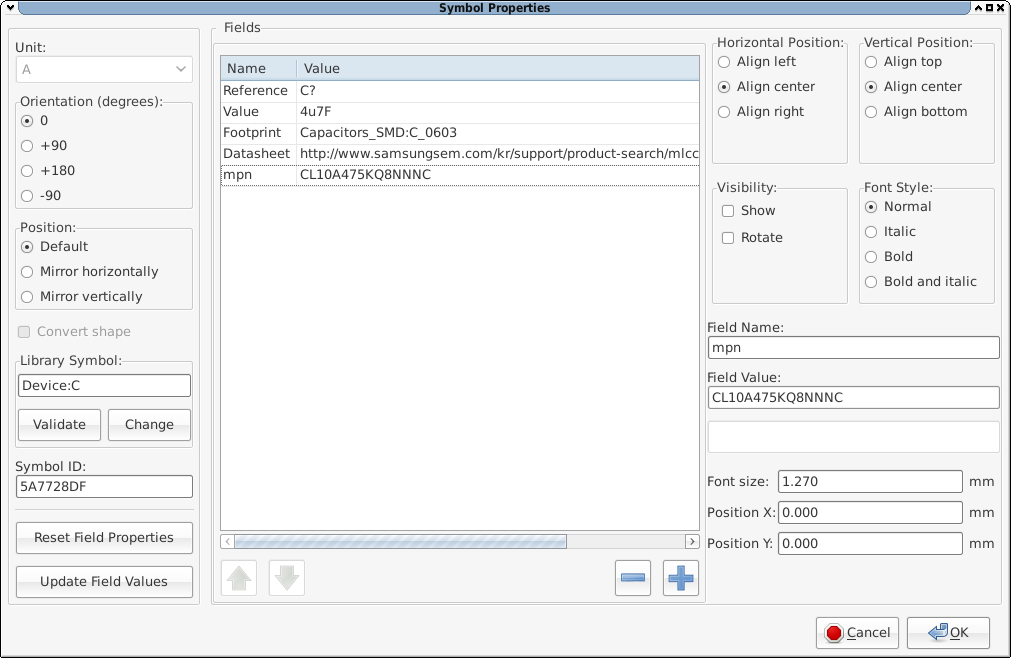
\includegraphics{chapter11/6-EditSymbolFinished.png}
	\caption[Symbol Properties]{
		Editing the Symbol Properties.
		}
	\label{fig:symbprop}
\end{figure}

It is a good idea to add the MPN to each part while you are building the circuit.
This ensures that your schematic matches the reality of which parts are available to you.
Often, if you design a schematic without MPN, you will find at the end that you need to substitute a number of components due to availability issues, incompatibility or other problems.
Replacing components in complex circuits can often have knock-on effects when the changes cascade from one system to the next.

When adding parts, I like to think in terms of groupings.
These groups of components are natural starting points for subsheets in a schematic.
Most boards will have some input and some output.
The input might be external connections or a board mounted sensor or user buttons.
The output might likely be external connections or a display or a motor.

Whatever the inputs and outputs, I find it useful to group these sections separately and add the components to them individually.
In each sheet, I will add components in a roughly circular pattern around a central component.
Often, sheets will have one or two of these `pools' of component groupings.

\section{Connections}

Once you have your components in place on your schematic, you'll need to tell Eeschema how you would like them to connect.
Connections can be made directly pin-to-pin\sidenote{Most designers will only use this sort of shortcut in the case of a power pin; either voltage supply or ground reference.} or via an intermediate wire.
Connections can also be implied by the use of labels to denote which wires are electrically connected without being graphically connected.

There is no hard and fast rule for how to lay out the connections between pins.
Just as there are no rules set in stone for how one should construct a sentence or paragraph or novel.
But just as there are novels that are enjoyable and those that are not, so too are there schematics that are informative, enlightening and helpful.
And those that are not.

General do-rules for good schematic design
\begin{enumerate}
\item Group schematic items by function.
\item Use global power labels for power connections.
\item Label any wire that goes between active components.
\item Use busses for groups of functionally related connections.
\item Use symmetry when laying out similar parts and functions.
\end{enumerate}

General do-\textbf{not}-rules for good schematic design
\begin{enumerate}
\item Do not cross unconnected wires more than absolutely necessary.
\item Do not be cramped.
\item Do not draw wires that are not horizontal, vertical or 45$^{\circ}$. 
\end{enumerate}

\subsection{Wires}

\begin{figure}
	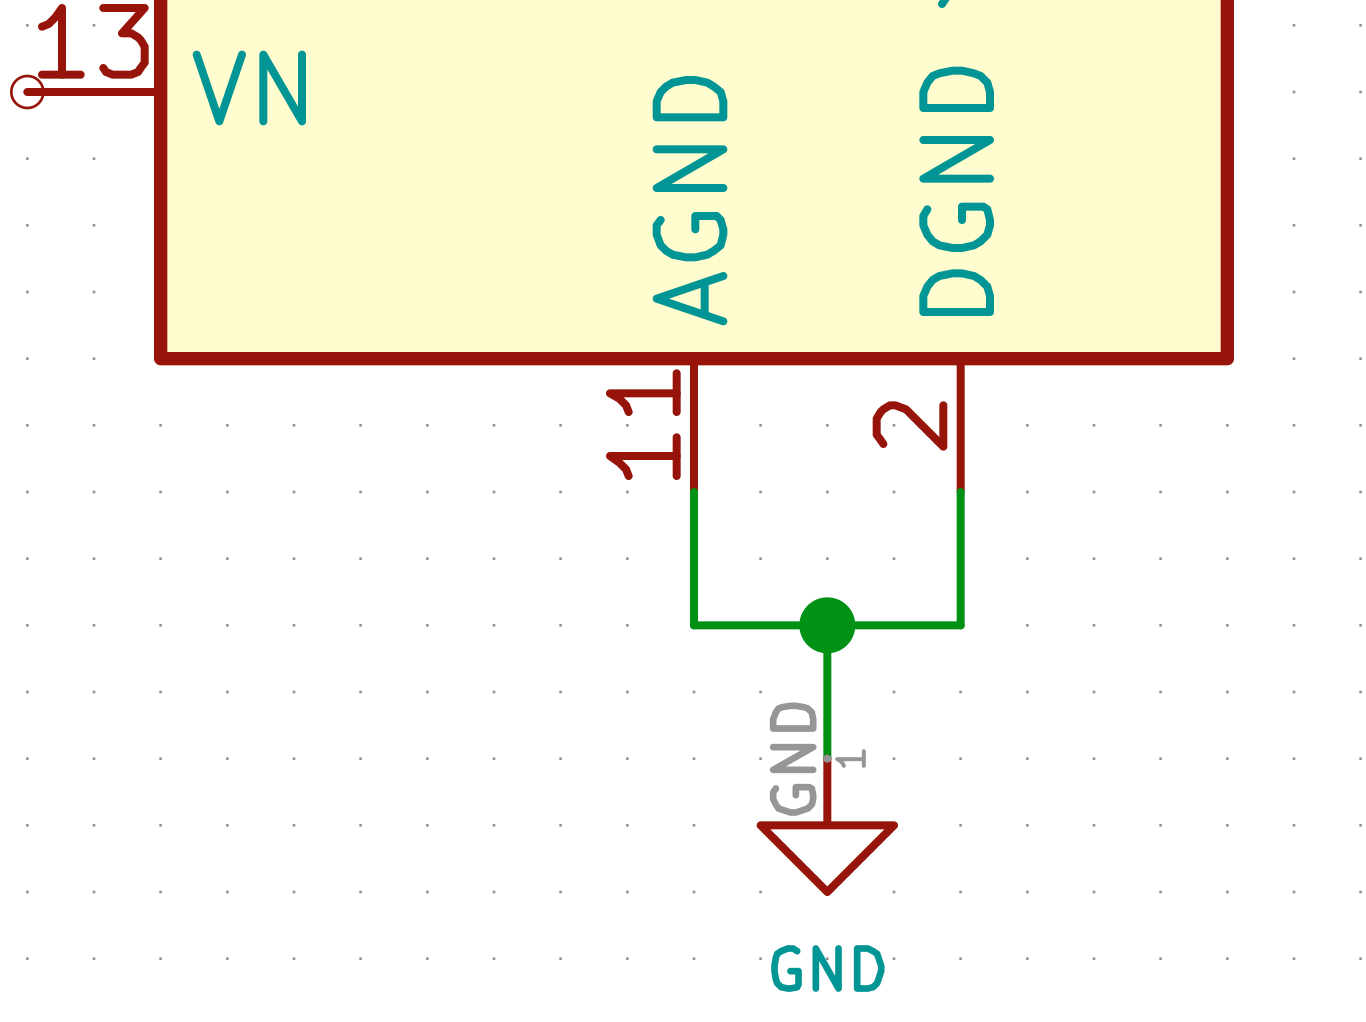
\includegraphics[width=0.8\textwidth]{chapter5/3-multiple-wires.png}
	\caption[Wire connection between pins]
	{
		The wires form an electrical connection between pins 2, 11 and the ground symbol.
		The junction (green circle) indicates an electrical connection between all three wires at the junction location.
	}
	\label{fig:multiple-wires}
\end{figure}

Wires form the basic connections in KiCad.
Any two points on the schematic with a wire between them are connected to the same net in the netlist.
In Figure \ref{fig:multiple-wires}, the wires connect pins 11 (AGND) and 2 (DGND) of the IC with each other and with pin 1 of the GND symbol.

\subsection{Busses}

Busses are similar to wires in that they can connect signals.
The key difference is the busses can carry multiple signals in a single line.

KiCad treats busses slightly differently than other schematic capture programs.
Busses in KiCad can only be used to connect numbered signals.
Specifically, the numbered signals need to follow the convention \textsc{NAME}\textbf{X} where \textsc{NAME} is the signal name and \textbf{X} is the signal number.
Examples of correct signal numbering for KiCad are \textsc{DIO1}, \textsc{DIO2}, \textsc{DIO3}.
Signal names that cannot be bussed are \textsc{SCK}, \textsc{SDI}, \textsc{SDO}.
You also cannot bus signals like \textsc{CS0}, \textsc{SPI1}, \textsc{SPC2}

\subsection{Labels}

Labels act as implicit connections between points on the schematic.  
Labels can be attached to wires, pins and busses.

When placed on a wire or a pin, the label will assign a name to the electrical connection.
Placing the same label on a second wire or pin will connect the first and the second.

There are three types of labels in KiCad.
They differ in their scope as well as their precedence.

\begin{marginfigure}
	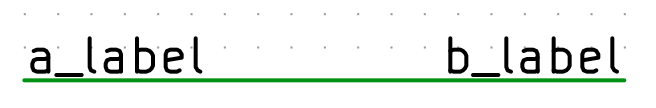
\includegraphics{chapter5/4-multiple-labels.png}
	\caption[Local Labels]{
		Two local labels are joined by a single wire.  
		They both connect to the same named net.
		The net name is decided by label precedence.
	}
	\label{fig:locallabels}
\end{marginfigure}
\paragraph{Local Labels} 
The most basic and lowest precedence label in Eeschema is called a Local Label.
An example of a local label is shown in Figure \ref{fig:locallabels}.
This label appears as unadorned text with the connection point at the bottom of the beginning or bottom of the end of the text, depending on its orientation.
Wires can connect using these labels only on the same schematic sheet.
You can reuse local label names across different sheets and hierarchy levels without connecting the wires.

In Figure \ref{fig:locallabels}, the net will be named according to alphabetical order if there are no other labels connected.
Therefore, in the netlist, this net will be referred to as '\textbf{a\_label}'.

\begin{marginfigure}
	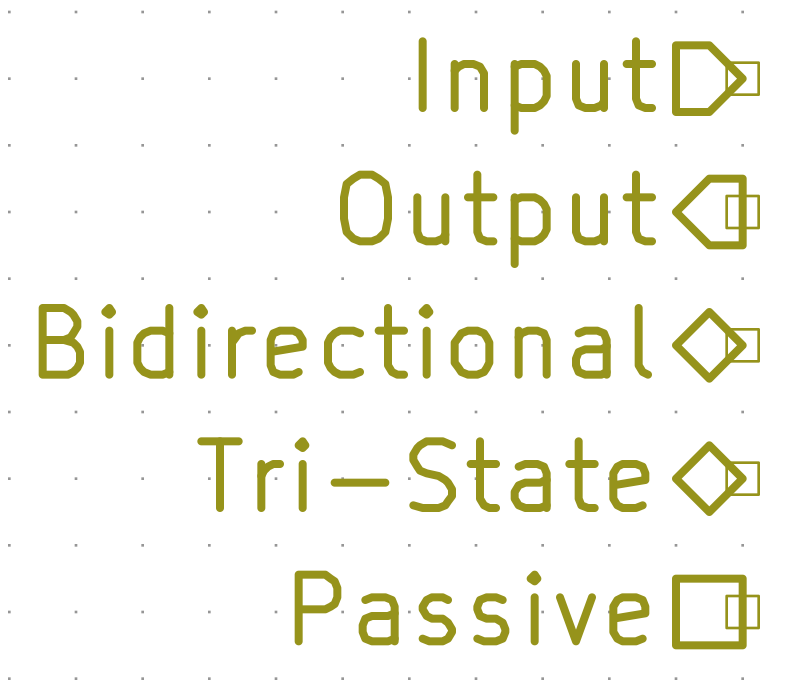
\includegraphics{chapter5/5-hlabel-types.png}
	\caption[Hierarchical Labels]{
		The five graphical types of hierarchical labels are shown here.
	}
	\label{fig:hlabel-types}
\end{marginfigure}
\paragraph{Hierarchical Labels} The next type of label in precedence is called a Hierarchical Label.
Hierarchical labels connect both signals on the same schematic sheet as well as those signals in the hierarchy's parent schematic sheet.

To create a hierarchical label, you must link both the parent sheet and its child sheet together with the same label name.
This is done by first creating the hierarchical label in the child sheet (Hotkey default: \textbf{H}) and then, using the ``Import Hierarchical Pin'' tool, clicking on the child's sheet from within the parent sheet.

\begin{marginfigure}
	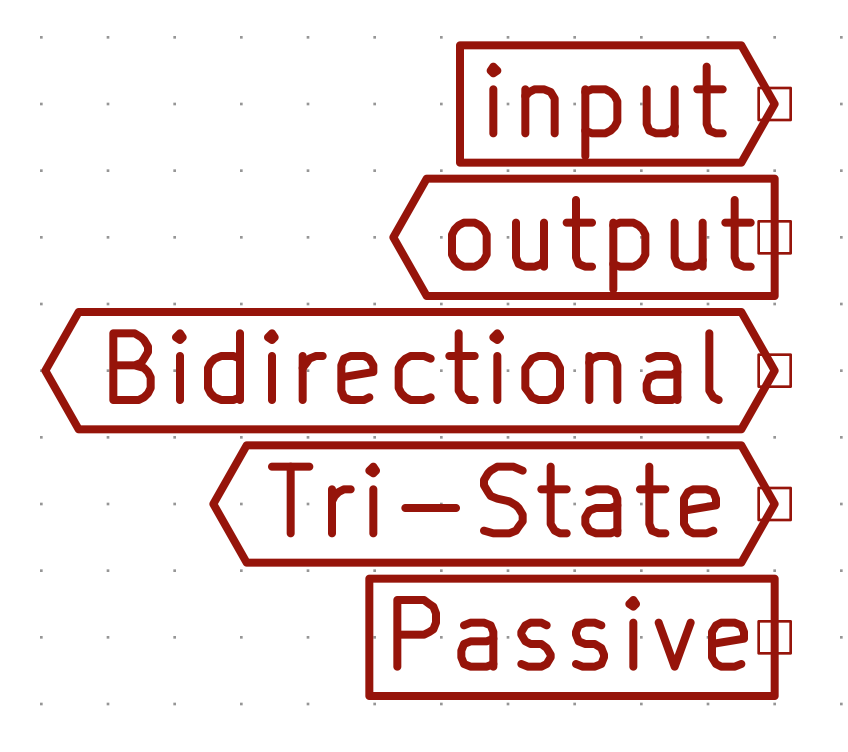
\includegraphics{chapter5/6-glabel-types.png}
	\caption[Global Labels]{
		The five graphical types of global labels are shown here.
		Note that there is no inherent difference in the type of label other than symbol.
		The symbol is a graphical reminder of what type of signal is used at that point in the schematic.
	}
	\label{fig:glabel-types}
\end{marginfigure}
\paragraph{Global Labels} The global labels are similar in appearance to the hierarchical labels.
They exist at the highest precedence in the schematic.
The net name can only be used for a single network in the entire schematic and will overwrite other netnames where it is connected to them.

\subsection{Junctions}
\begin{marginfigure}
	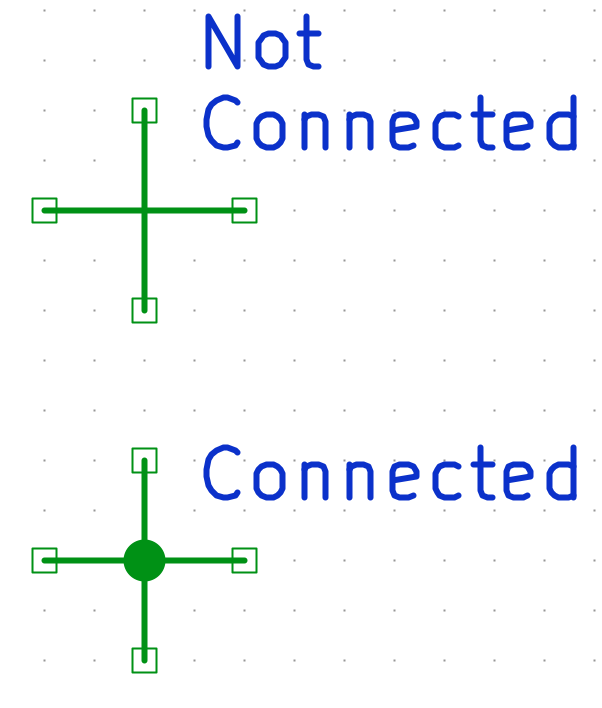
\includegraphics{chapter5/7-junctions.png}
	\caption[Wires with and without a junction]{
		The junction shown connects the two wires.
		Otherwise, they will form two distinct nets.
	}
	\label{fig:junctions}
\end{marginfigure}
A junction connects two wires into a single net.
Wires that merely touch as shown in the top of Figure \ref{fig:junctions} will not connect to the same net.
Adding a junction to the point where the pins connect will join the wires together in the same net.

At each junction, a wire is broken into two segments (before and after the junction).

\subsection{No Connects}
\label{sec:noconnect}
Every pin in your schematic should be explicitly connected to at least one other, compatible pin.
If they are not, the Electric Rules Check will raise an error.
Sometimes, however, this is not the behavior that you intend.
For example, if you use a hex inverter like \textbf{SN7404} but only need 5 of the six elements, you will want to explicitly show the Electrical Rules Check that the sixth element output pin should not be connected on your circuit.

The no-connect symbol can be placed on pins to indicate that you intend to leave the pin electrically unconnected.

\subsection{Hierarchical Pins}


\section{Electrical Rules Check}

\newthought{The Electrical Rules Check (ERC)} is one of the most useful and, to those just learning Eeschema, confusing aspects of schematic design.
ERC acts as a check against basic mistakes in circuit design.
It tests how you have connected component pins together, warning or giving an error when conflicting types are connected or left floating.
It also tests for label names that are conflicting or differ only by the capitalization.

Because ERC is so useful and confusing, we'll spend a bit of covering the options as well as work-arounds for when you \textit{really} want to do something that ERC doesn't like.
We'll cover the pin types in the same fashion as the ERC options window ? that is by working through potential combinations without duplication.
To read the various connection combinations in the ERC options, you should find your first pin type in the left-hand column.
Then, follow all of the connection options to the right by looking at the column label.
Once you reach the identity combination (e.g. Intput-Input or Passive-Passive), follow the remaining combinations vertically down the column and match the options by looking at the row label.

\paragraph{No Connection} In ERC, No Connection means a dangling connection.
That is, a pin that isn't connected to another pin \textbf{and} doesn't have a no connect symbol attached to the end.
To get rid of these errors, you need to connect the pin or explicitly show that it shouldn't have a connection by attaching a no connect symbol as discussed in Section \ref{sec:noconnect}.

\paragraph{Input Pin} The Input can connect to all other pin types except Unspecified pins, which throw warnings.
The logic is that input pins will typically be high-impedance, therefore they should not interfere with the operation of other pins.
Not listed in the options is the additional ERC check that each net have at least one non-input pin.
If your net is purely high-impedance input pins, then nothing will set the potential voltage.

\begin{marginfigure}
	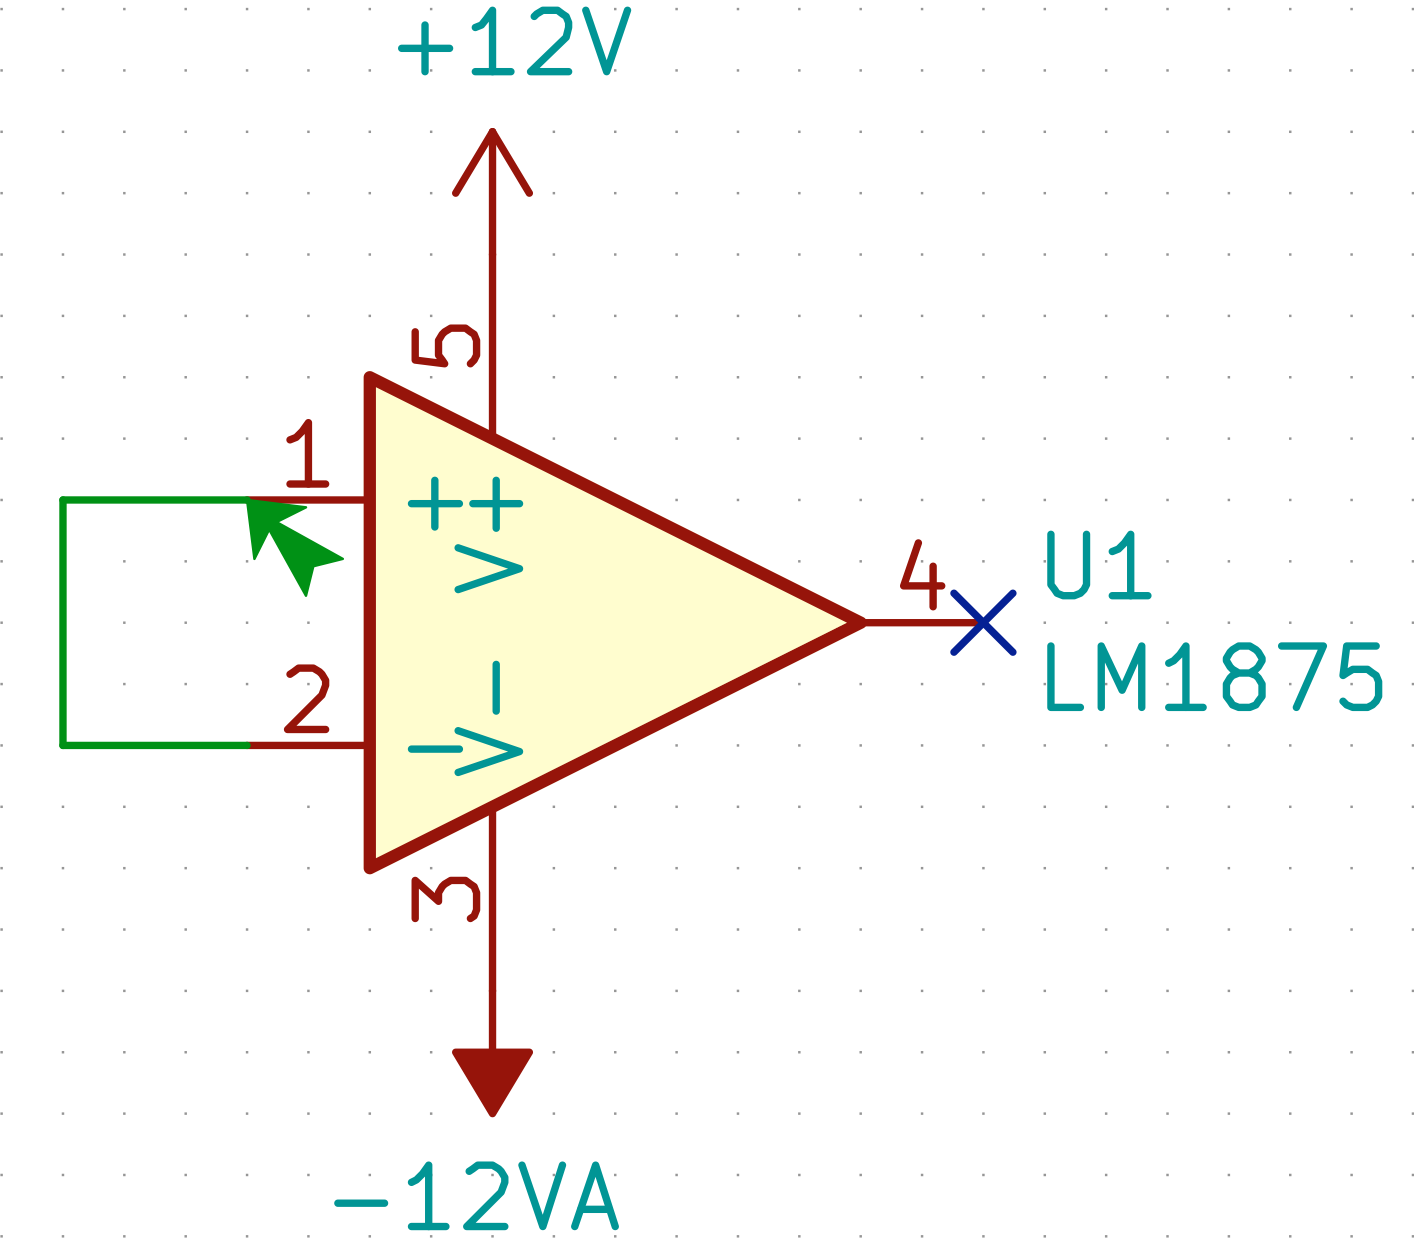
\includegraphics{chapter5/8-inputpinERC.png}
	\caption[Error on input pins]{
		The green arrow shows the result of an ERC for this simple circuit.
		Here, the inverting and non-inverting inputs are both high-impedance input pins.
		The ERC reports ``\textbf{ErrType(3): Pin connected to some others pins but no pin to drive it.}''
	}
	\label{fig:inputerc}
\end{marginfigure}
An example of this is shown in Figure \ref{fig:inputerc}.
The ERC options do not allow you to disable this error.

However, there might be a case where you want to allow two input pins to be the only ones on a net.
While these should be the exception rather than the rule, it can be helpful to designate this net as allowed.

A simple bypass is shown in Figure \ref{fig:inputerc-fixed}.
The passive pin on the testpoint tells the ERC that the net is acceptable as-is.
The testpoint does need to be annotated, as all symbols do on the schematic.
By manually prefixing the symbol reference with a ``\textbf{\#}'', we indicate that there is no footprint associated with the test point.
The ``\textbf{\#}'' indicates that the symbol is a flag rather than an actual component.
If you don't like having the test point colocated with your pins, you can always use a label to attach the flag to the net at a spot where it doesn't detract from your circuit.
\begin{marginfigure}
	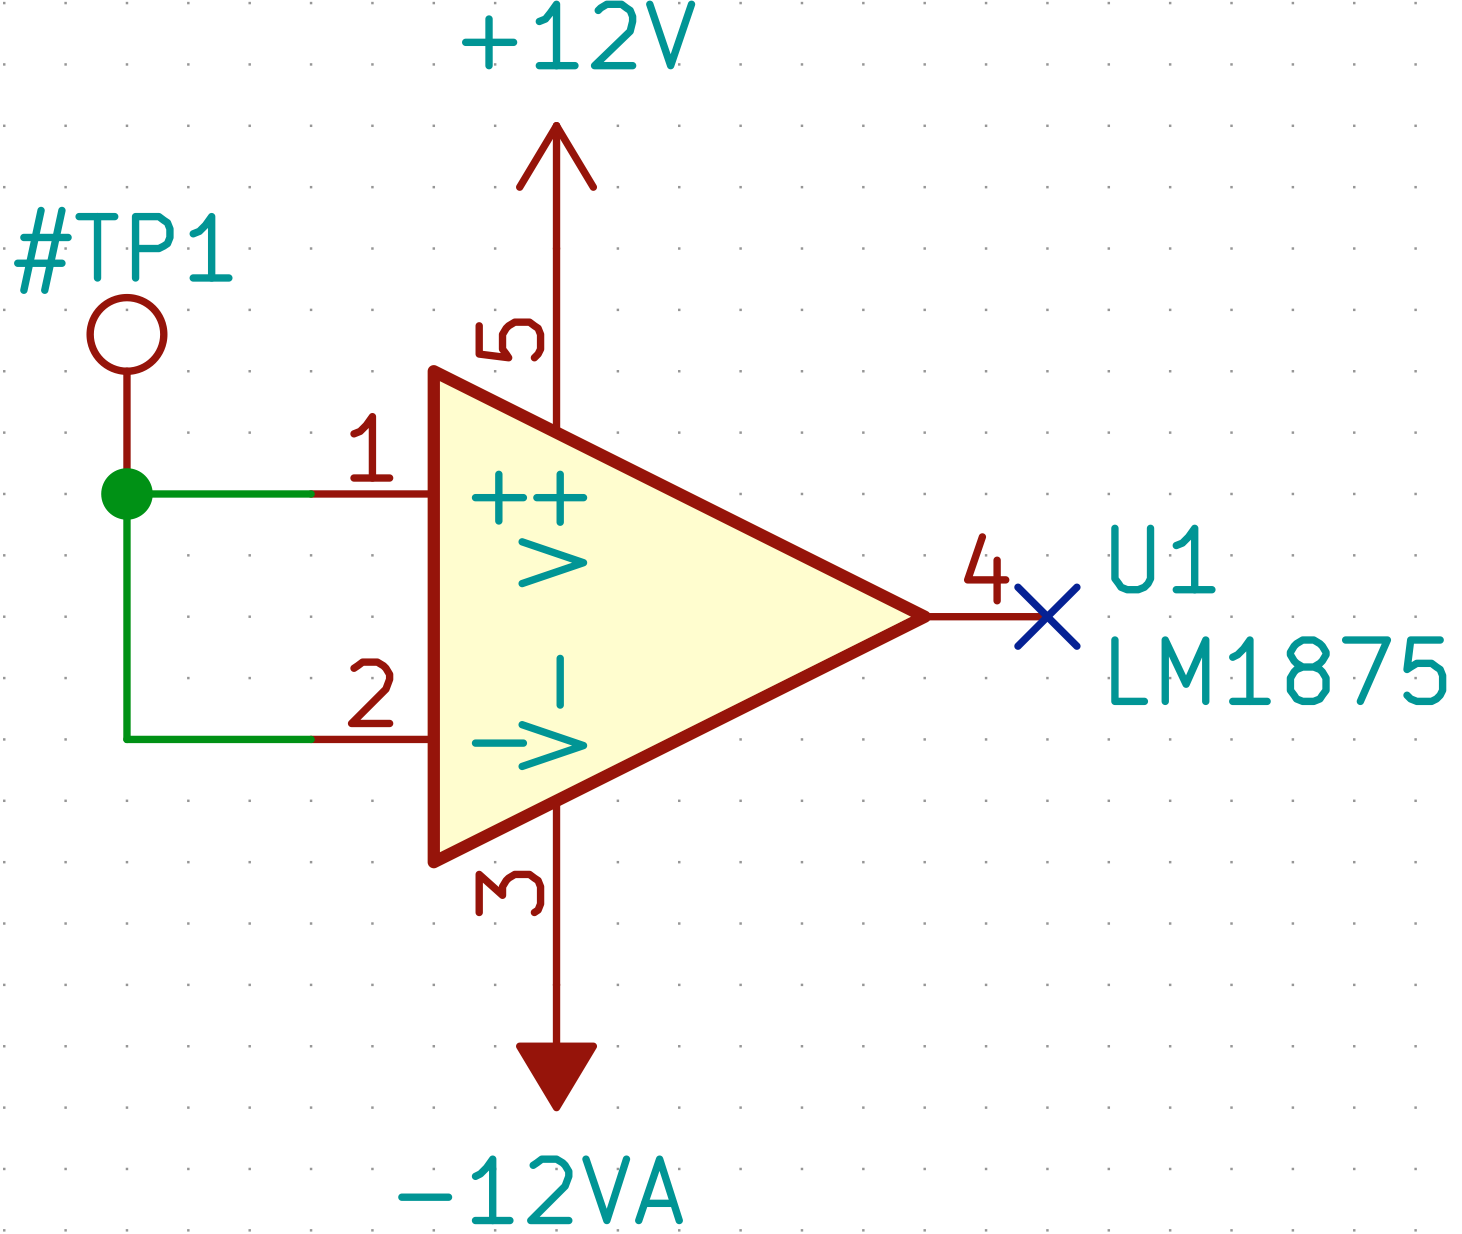
\includegraphics{chapter5/9-inputpinERC-fixed.png}
	\caption[Allowing only input pins]{
		The addition of a test point on the net resolves the ERC error from Figure \ref{fig:inputerc}.
		This adds a passive pin to the network, bypassing the ERC error.
		The name begins with ``\textbf{\#}'' to prevent a footprint from being placed on the schematic.
	}
	\label{fig:inputerc-fixed}
\end{marginfigure}

\paragraph{Output Pin} Pins designated as output actively set their own voltage potential.
By default, ERC allows these to connect to input, power input, bidirectional and passive pins without error.
Connecting an output pin to a Tri-State pin or an unspecified pin will generate a warning and connecting an output pin to any other type of output pin, including open collectors and open emitters is an error.

The logic behind warning when connecting an output pin to a tri-state pin is that it might not allow the tri-state pin to reach its third state (disconnected).
Some output pins, however, will go into a high-impedance state when their IC is disabled, either by a separate pin or disconnecting power.
Or you might not need access to the pin's third state and therefore are perfectly happy to allow it to connect to an output pin.

The logic behind throwing an error when there are multiple outputs on the same net is that the net may be driven to different voltages by the different outputs.
When this happens, the copper trace between the outputs is the only impedance, leading to potentially large current draws and damage.
While this is almost always a bad thing, there are cases where you might want more than one output connected to the same net.
\begin{marginfigure}[-2in]
	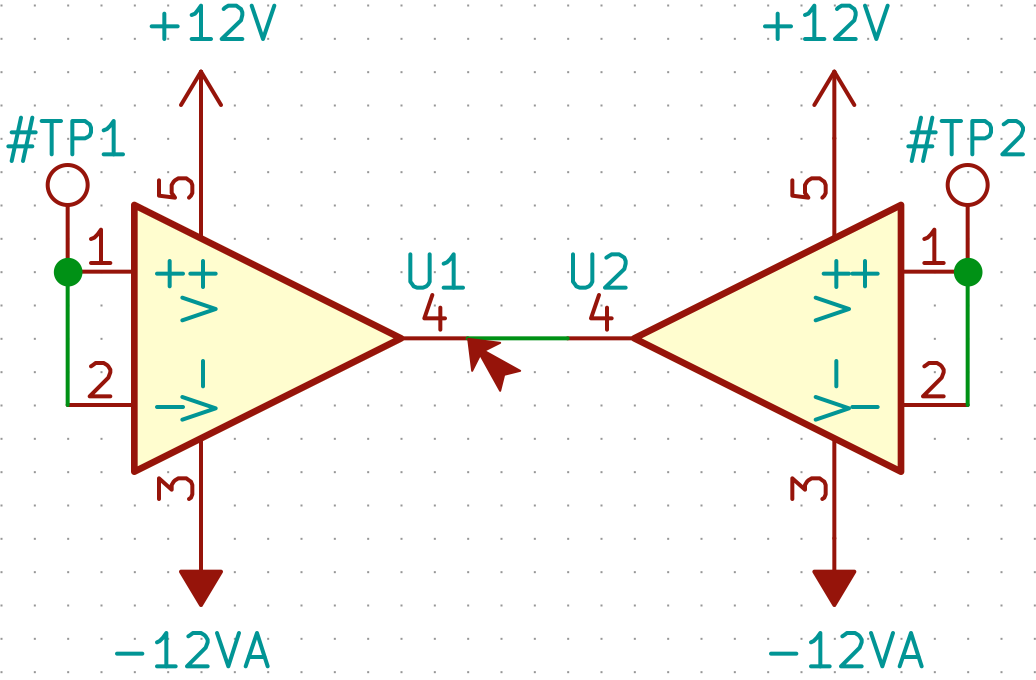
\includegraphics{chapter5/10-outputpinERC.png}
	\caption[Error connecting output pins]{
		The red arrow shows that we have a pin conflict in the ERC.
		The ERC error message is ``\textbf{ErrType(5): Conflict problem between pins. Severity: error}''.
	}
\end{marginfigure}
To accomplish this, we employ a net tie.
You will find these symbols in the ``device'' library.
\sidenote{
	You could accomplish the same action by using any two-terminal passive component such as a resistor or inductor but this causes unnecessary confusion in your schematic.  
	Net ties are preferred as they indicate a component that exists only as a schematic and copper item.
}
\begin{marginfigure}
	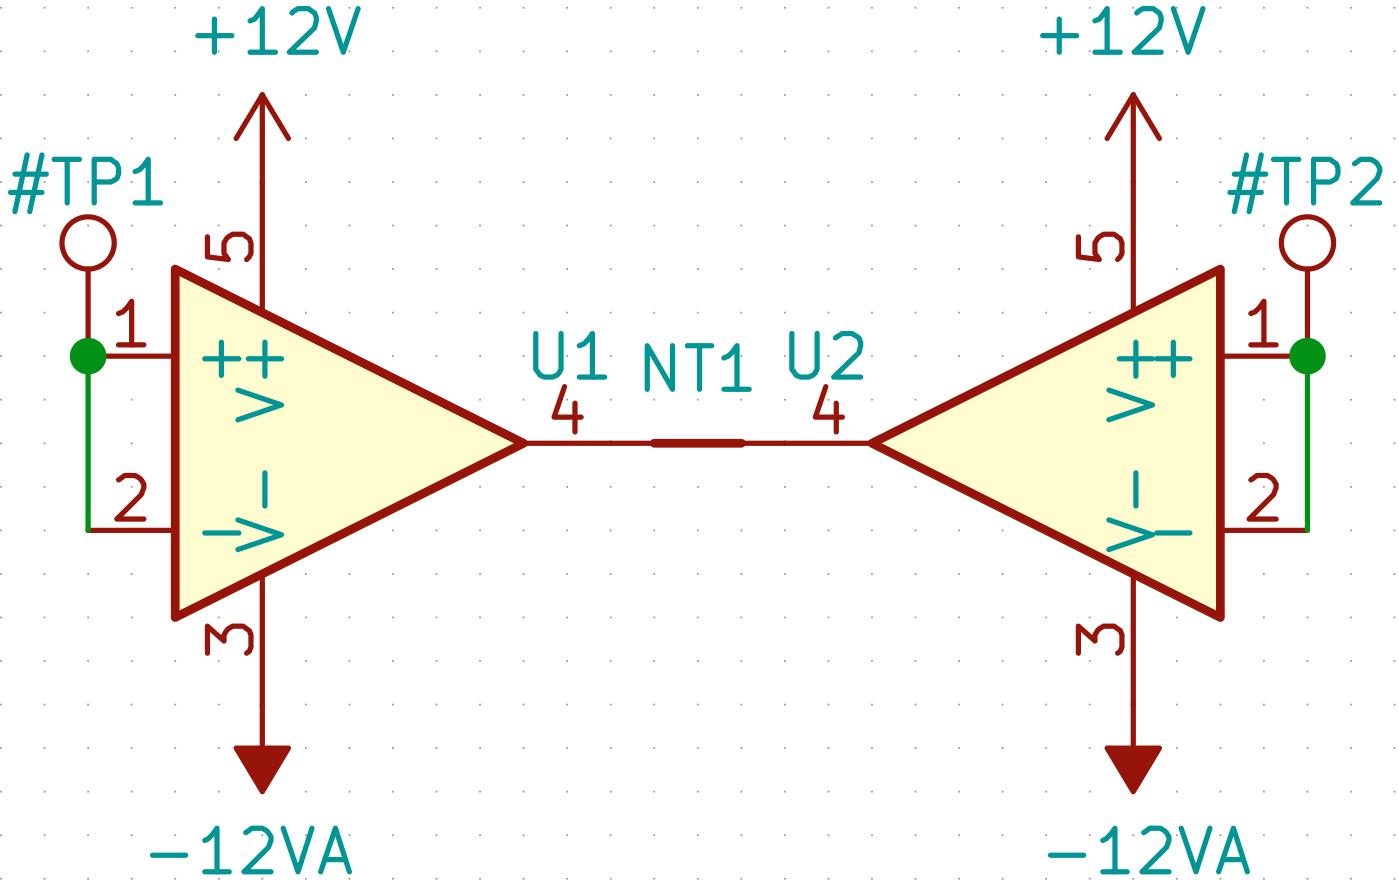
\includegraphics{chapter5/11-outputpinERC-fixed.png}
	\caption[How to connect output pins]{
		By placing a passive net tie between the two output pins, the ERC error is resolved.
	}
	\label{fig:nettie}
\end{marginfigure}
By placing a net tie between the two output pins as shown in Figure \ref{fig:nettie}, the output pins each connect to a passive pin on the net tie, resolving the ERC error.
On the PCB, a net tie footprint is two overlapping copper pads.
You can create your own to get a specific copper width or use one of the pre-defined ones in the KiCad footprint library.

\paragraph{Bidirectional Pin} The Bidirectional pin will issue a warning when directly connected to low impedance output pins including power output, open collector and open emitter pins.
If you wish to suppress this type of error for a single connection, you can employ the net tie workaround as shown in Figure \ref{fig:nettie}.
It is generally considered good design to employ an actual resistor that will limit the current potentially sunk by the bidirectional pin, should it accidentally be set to output when there is a power output on the same net.
For example, if your bidirectional pin can sink up to 20 milliampere of current and it is meant to connect to a power output of 15 volts, safe design would add a resistor of at least 750 ohms between the bidirectional pin and the power output pin.
As the designer, however, you will need to take into account all of the other factors that might be affected by the addition of this resistor.

\newthought{The remaining ERC connection combinations} take the same form as the three we've discussed above.
Warnings are issued for connections that \textit{might} be unintentional.
Errors are issued for connections that \textit{usually} are unintentional or problematic.
Each of the ERC checks can be changed from their default to valid (green), warning (yellow) or error (red).
Changing in the ERC options will affect the entire project.

\begin{quote}
	\itshape Note that, of the ERC options, only the option to test for similar labels is saved.
	All other options are reset at each KiCad session, so you will need to re-initialize them between runs.
	The test for similar labels option is saved in the KiCad project file and therefore will need to be unset for each KiCad project in which you want it disabled.
\end{quote}

\section{Graphical Elements}
Adding an image to your schematic can be helpful in documenting a schematic, branding your work or just an attractive decoration.
Eeschema supports adding many common bitmap image formats including PNG, JPG, BMP, PIC and others.
Once added to your schematic, the image can be moved, rotated, flipped and rescaled.
It can also be converted to greyscale, however, at the moment, this is a one-way operation, so use with care.

\section{Annotation}

Before exporting your circuit diagram or even running the ERC, you will need to assign unique names to each of the components in your schematic.
This process is called ``Annotating''.
When you first place a new symbol or duplicate an existing symbol in Eeschema, the Reference field is suffixed with a ``?''.
During annotation, this question mark is replaced by a sequential number\sidenote[][-36pt]{The sequence of the number can optionally be set to start at the beginning of the hierarchy or at a multiple (100x, 1000x) of the sheet number}, giving each component in your schematic a unique reference.

\begin{figure}
	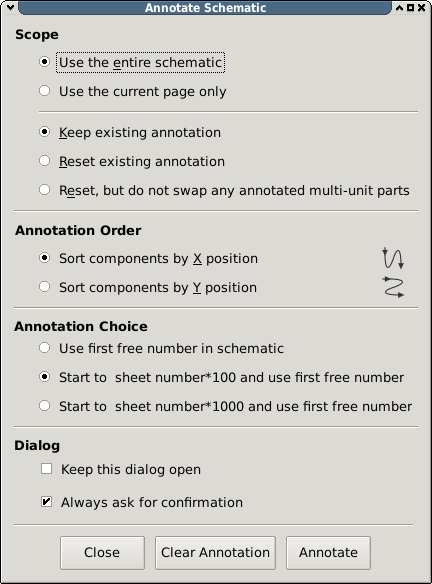
\includegraphics[width=0.5\textwidth]{chapter11/60-Annotate.png}
	\caption[Annotation Options Window]{The annotation options window allows you to clear and complete the annotation of a schematic.  You will need to do this whenever you add a new component to your schematic before you can use it.}
	\label{fig:annotate}
\end{figure}



\section{Schematic Editor Examples}
\subsection{Example 1: Single Page Schematic}
\subsection{Example 2: Hierarchical Schematic}